\documentclass{article}
\usepackage{pdfpages}
\usepackage{graphicx}
\usepackage{float}
\usepackage{listings}
\usepackage{color}

\definecolor{dkgreen}{rgb}{0,0.6,0}
\definecolor{gray}{rgb}{0.5,0.5,0.5}
\definecolor{mauve}{rgb}{0.58,0,0.82}




\begin{document}
\lstdefinelanguage{glpk}{
	keywordstyle=[2]\color{blue},
	keywordstyle=[3]\color{purple},
	morekeywords={param, set, var, s.t.},
	keywords=[2]{data, end},
	keywords=[3]{maximize, minimize},
	sensitive=True,
	morecomment=[l][\color{darkgray}]{\#},
}
\lstset{
	language=glpk,
	showstringspaces=true,
	numbers=left,
	numberstyle=\tiny,
	columns=fixed,
	breaklines=true,
	tabsize=4,
}






\title{Modelos y Optimizaci\'on I\\ \large{Trabajo pr\'actico: Ejercicio PLC}}
\author{De Valais, Ezequiel\and	Rozanec, Matias}
\date{Septiembre 2017}
\maketitle
\newpage
% FIN PRESENTACION 
\tableofcontents
\newpage
% Consigna
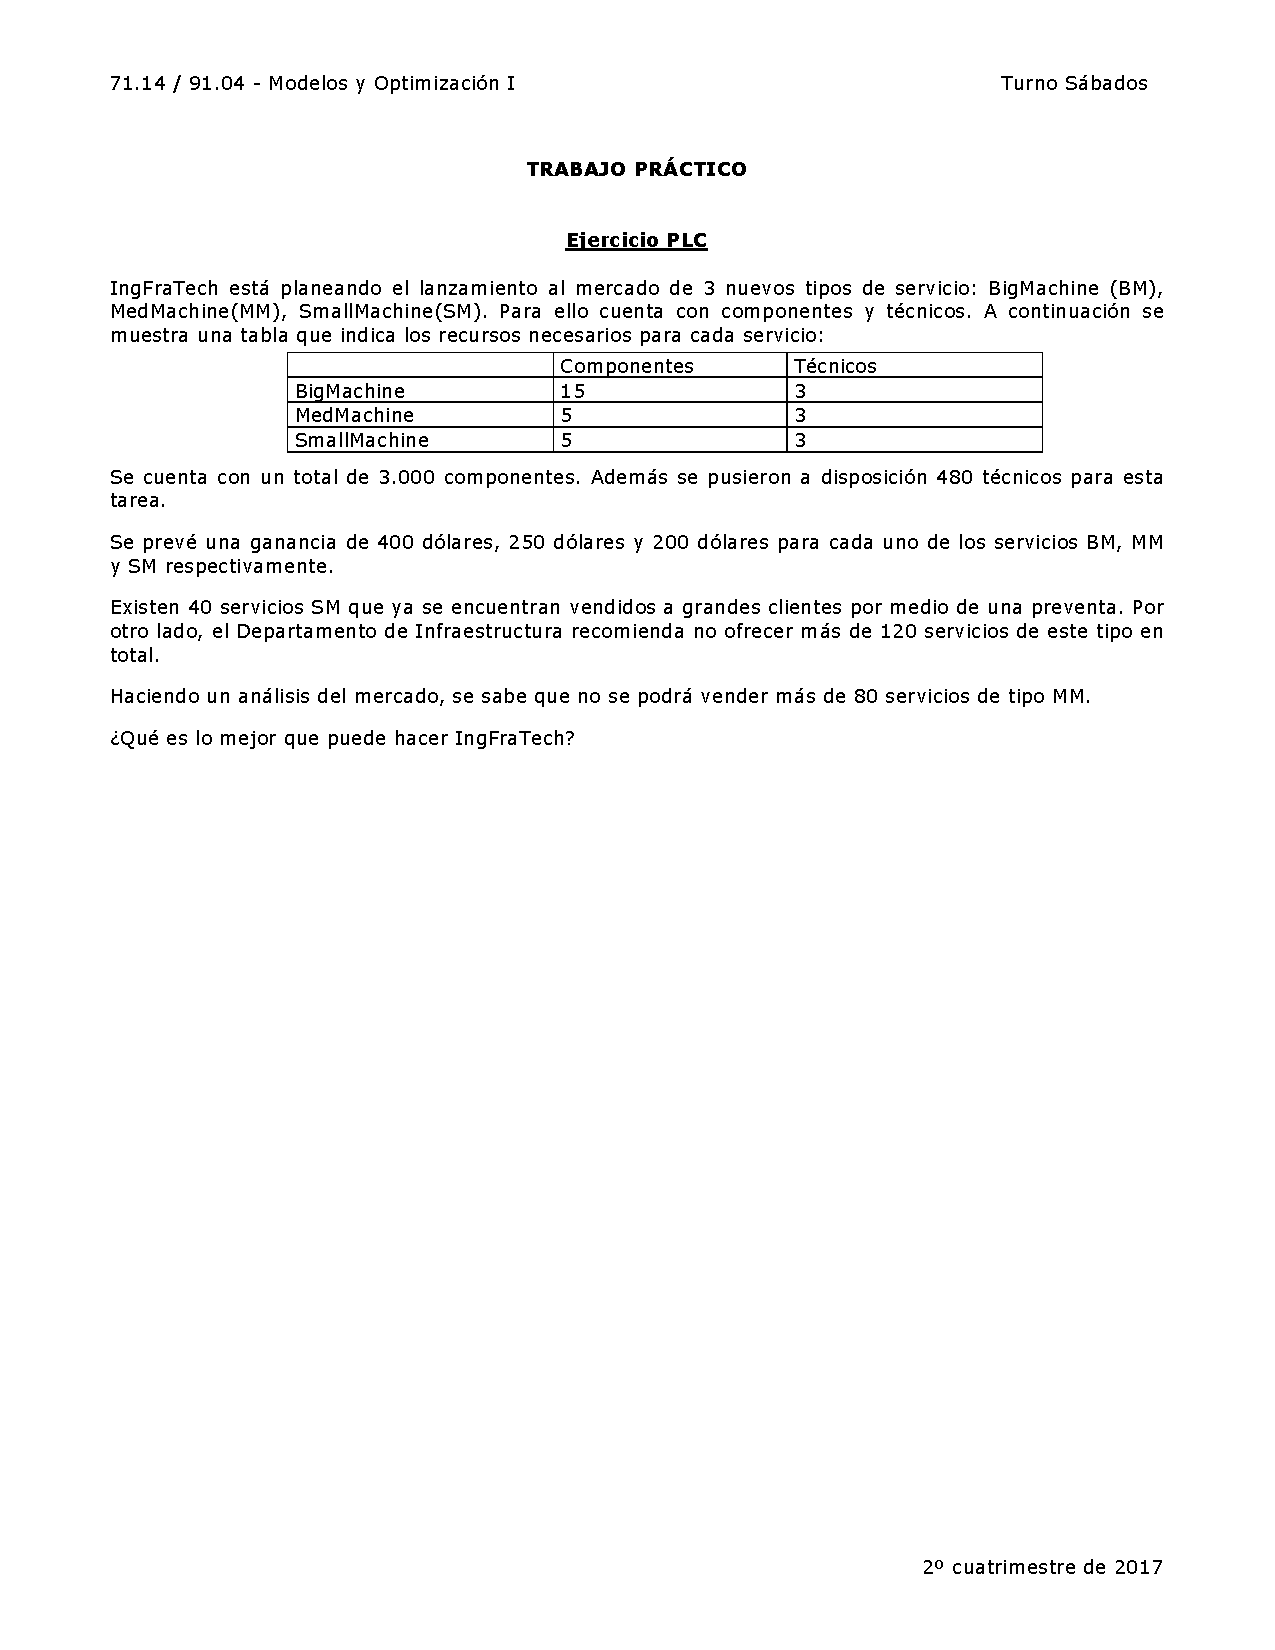
\includepdf{EnunciadoPLC.pdf}
\newpage

% Resolucion
\part{Descripci\'on de la situaci\'on problem\'atica}
En el presente enunciado se nos presenta el caso de una empresa que desea incluir 3 nuevos servicios. Seg\'un el enunciado, la empresa ya ha realizado un estudio de mercado, a partir del cual tiene c\'alculos aproximados de ventas m\'inimas y m\'aximas para algunos de los nuevos servicios a ofrecer. A esto se le suma una cantidad de servicios vendidos en modo preventa. 
Seg\'un el enunciado, para poder ofrecer los nuevos servicios se necesitan tanto componentes como te\'cnicos capacitados. Contando con la informaci\'on de:
\begin{itemize}
	\item cantidad de componentes y t\'ecnicos
	\item estudio de mercado
	\item ganancia por servicio vendido
\end{itemize}
se nos pide estudiar c\'omo deber\'ia proceder la empresa. \\
Se trata de un problema de mezcla y armado.\\
A continuaci\'on, se incluye un diagrama que representa de forma simple el escenario descripto. 
% Diagrama
\begin{figure}[h!]
	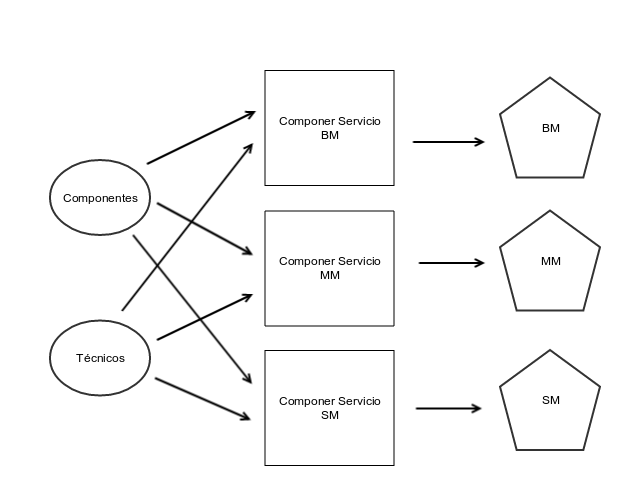
\includegraphics[scale=0.5]{tp_myo.png}
\end{figure}

\part{Objetivo}
Determinar la cantidad de servicios BigMachine(BM), MediumMachine(MM) y SmallMachine(SM) a componer durante un per\'iodo de tiempo para maximizar la ganancia.

\part{Hip\'otesis y supuestos}
\begin{itemize}
	\item Los gastos ya se encuentran considerados dentro de los estimados de ganancia
	\item Los productos de preventa generan la misma ganancia que los productos post lazamiento
	\item No hay inflaci\'on 
	\item La ganancia no var\'ia
	\item Los componentes van a estar disponibles durante todo el per\'iodo (no se rompen).
	\item Los t\'ecnicos van a estar disponibles durante todo el per\'iodo (no se enferman ni renuncian).
	\item Todos los servicios preparados se venden.
	\item Pueden quedar t\'ecnicos o componentes sin utilizar/asignar y estos no generan ning\'un gasto.
	\item No hay otras limitacines que las del enunciado.
	\item Excedentes no se venden a inter\'es.
	\item El pago es recibido al momento de vender el servicio y al contado.
	\item No se consideran feriados.
	\item Los t\'ecnicos pueden ser asignados a cualquier servicio de forma indistinguible.
\end{itemize}


\part{Definici\'on de variables, incluyendo unidades}
\begin{itemize}
	\item BM: Cantidad de servicios[s] BM a componer en un periodo [t]. [s/t]
	\item MM: Cantidad de servicios[s] MM a componer en un periodo [t]. [s/t]
	\item SM: Cantidad de servicios[s] SM a componer en un periodo [t]. [s/t]
\end{itemize}

\part{Modelo de Programaci\'on Lineal Continua}
\begin{equation}
	SM \geq 0
\end{equation}

\begin{equation}
	MM \geq 0
\end{equation}

\begin{equation}
	BB \geq 0
\end{equation}
\section{L\'imite Ventas}
\begin{equation}
	SM [s/t] \leq 120 [s/t]
\end{equation}
\begin{equation}
	MM [s/t] \leq 80 [s/t]
\end{equation}

\section{Preventa}
\begin{equation}
	SM [s/t] \geq 40 [s/t]
\end{equation}

\section{L\'imite Componentes} 
\begin{equation}
	BM [s/t] * 15 [c/s] + MM [s/t] * 5 [c/s] + SM [s/t] * 5 [c/s] \leq 3000 [c/s]
\end{equation}

\section{Limite T\'ecnicos}
\begin{equation}
	BM [s/t] * 3 [tec/s] + MM [s/t] * 3 [tec/s] + SM [s/t] * 3 [tec/s] \leq 480 [tec/s]
\end{equation}

\part{Funcional}
\begin{equation}
	Z(max) = BM [s/t] * 400 [\$/s] + MM [s/t] * 250 [\$/s] + SM [s/t] * 200 [\$/s]  
\end{equation}

\part{Informe de los resultados obtenidos}
Analizando los resultados obtenidos, podemos observar que:
\begin{itemize}
	\item conviene vender 40 servicios SM
	\item conviene vender 0 servicios MM
	\item conviene vender 120 servicios BM
	\item de los 3000 componentes se usan solamente 2000
	\item estar\'an activos los 480 t\'ecnicos
	\item la restricci\'on correspondiente a los t\'ecnicos coincide con su l\'imite superior, y su marginal nos indica que si aumentara la cota superior en una unidad (que equivaldr\'ia a agregar a un t\'ecnico), se ganar\'ian \$133.333 m\'as. 
	\item la cantidad de ventas de SM coincide con la cota inferior. El marginal nos indica que si aumentara la restricci\'on en una unidad (o sea, si se deber\'ia producir una unidad m\'as de SM), el funcional disminuir\'ia en \$200.
\end{itemize}
Finalmente, el funcional nos indica que la ganancia sujeta a dichas observaciones ser\'ia maxima y de \$56000.


% APENDICE
\newpage
\part{C\'odigo fuente}
\section{Archivo del modelo}
\lstinputlisting[frame=single]{modelo_con_separacion/PLC.mod}

\section{Archivo de datos}
\lstinputlisting[frame=single]{modelo_con_separacion/PLC.dat}

\lstset{
	  basicstyle=\ttfamily,
}
\section{Archivo soluci\'on}
\lstinputlisting[frame=single]{modelo_con_separacion/PLC.sol}
\end{document}
